\section{Coarse-to-Fine Semantic Segmentation From Image-Level Labels}

\begin{flushleft}
    \author{
    Longlong Jing,
    Yucheng Chen,
    Yingli Tan,
    \emph{Fellow, IEEE}
    }
\end{flushleft}

\begin{center}
    \emph{IEEE TRANSACTIONS ON IMAGE PROCESSING, VOL.29, 2020}
\end{center}

\subsection{INTRODUCTION}
To obtain a semantic segmentation it is necessary to have an annotated 
training set. Semantic segmentation generally requires pixel-wise semantic 
annotation techniques which are time-consuming. To solve the annotation 
problem, weakly supervised and semi-supervised semantic segmentation 
methods have been proposed. Methods such as object-level labels and image-level 
labels are used to extract annotations. These annotations are useful for 
producing datasets useful for training a weakly supervised model, such as 
the one proposed. By training a weakly supervised semantic segmentation 
model, with the labels produced, the performances match those of the supervised 
methods. Unfortunately, methods such as object-level labels produce 
bounding boxes that are still not precise, so the use of the image-level labels 
method prevails. The dataset used is that of ImageNet where a category is 
associated with each image. The proposed model is able to generate as many 
segmentation masks as there are different objects belonging to different 
categories in each image. Network training takes place using information such as 
masks, images and labels of each category. An example of the coarse-to-fine 
mask produced by the model is the one shown in figure \ref{fig:semanticWork}.
\begin{figure}[htbp]
    \centering
    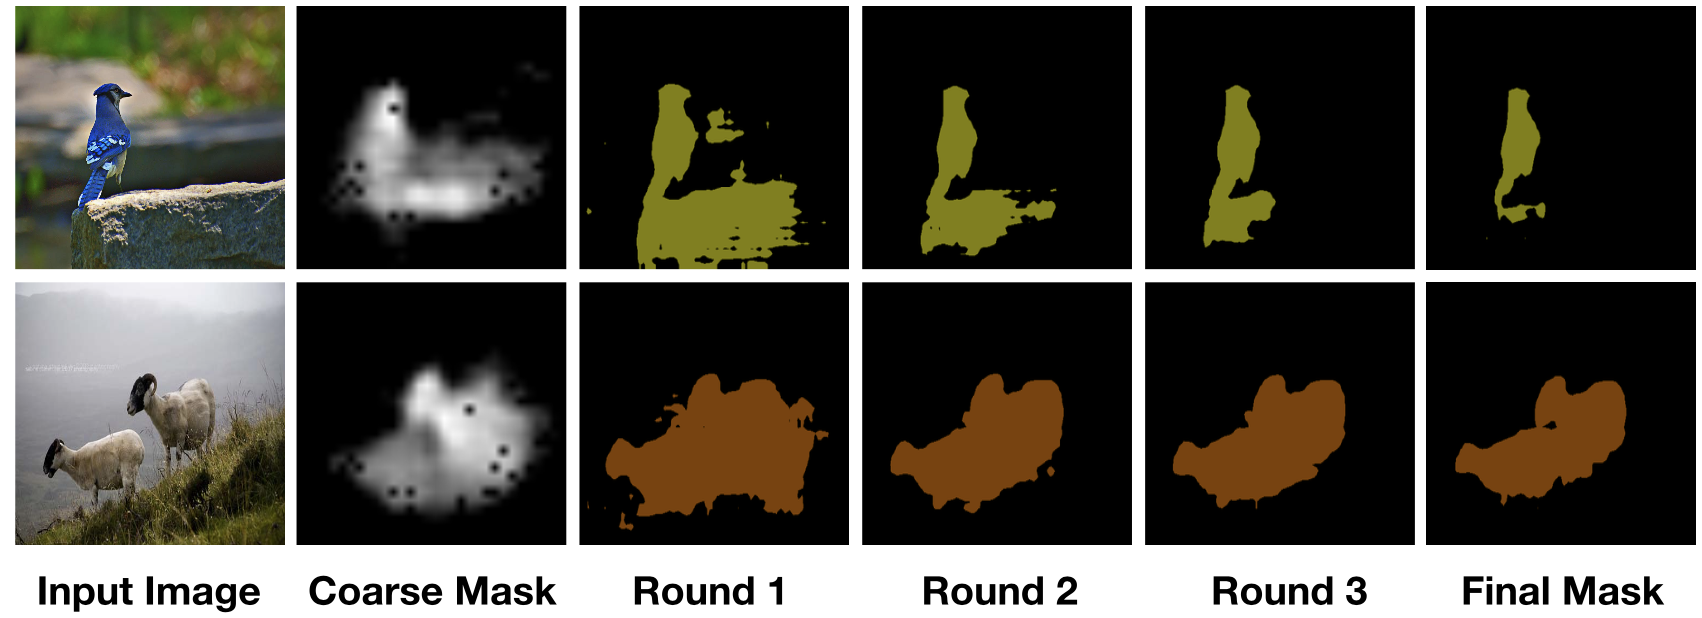
\includegraphics[width = 1 \linewidth]{images/paper6/work.png}
    \centering
    \caption{Example of semantic segmentation generated by the proposed method.}
    \label{fig:semanticWork}
\end{figure}